\documentclass{article}

\usepackage{Sweave}
\begin{document}
\Sconcordance{concordance:Ahern-permutation.tex:Ahern-permutation.Rnw:%
1 2 1 1 0 10 1 1 11 1 2 1 0 1 1 1 2 1 0 1 5 7 0 1 2 1 3 2 0 1 1 3 0 1 2 1 8 7 0 1 1 3 0 1 2 7 1}

%\SweaveOpts{concordance=TRUE}

\author{Christopher Ahern}
\title{Priming and permutation tests}

\maketitle

\section{}


\begin{Schunk}
\begin{Sinput}
> neg.data.full = cleanNegData("coding.cod.ooo")
> neg.data.full = tbl_df(neg.data.full)
> # Filter out tokens without do-support label, year, or type
> excluded.texts = c("CMBOETH", "CMORM", "CMNTEST","CMOTEST")
> # CMBOETH : translation of Boethius' "Consolation of Philosophy", which is notably stilted
> # CMORM   : Ormulum is very specific poetic format
> # CMOTEST, CMNTEST : Old and new testaments
> # Exclude tokens where 'ne' is contracted, appears in negative concord, or looks like predicate negation
> neg.data.full = neg.data.full %>% filter(! author %in% excluded.texts & exclude != "X") 
\end{Sinput}
\end{Schunk}

\begin{Schunk}
\begin{Sinput}
> # Plot individual documents
> neg.plot.auth = neg.data.full %>% group_by(year) %>% summarize(total=n(), ne=sum(neg.type=="ne", na.rm=TRUE)/total,not=sum(neg.type=="not", na.rm=TRUE)/total,ne.not=sum(neg.type=="both", na.rm=TRUE)/total)
> neg.plot.auth = melt(neg.plot.auth, id=c("year", "total"))
\end{Sinput}
\end{Schunk}

\begin{Schunk}
\begin{Sinput}
> # Plot points and smooth fits
> ggplot(aes(x = year, y = value, color = variable), data = neg.plot.auth) +
+   geom_point(aes(size = total), alpha = 0.5, position = position_jitter()) +
+   geom_smooth(aes(weight = total),method="loess", span=.5, se = FALSE, size=4) + # span=.5,
+   xlab("Year") +   ylab("Proportion forms") +   scale_size_area("N", max_size = 20) +
+   theme(text = element_text(size=30)) +   theme(legend.position="none") +
+   coord_cartesian(xlim = c(1090,1540)) +  coord_cartesian(ylim = c(-.1,1.1))
> ggsave('neg-plot-auth.pdf', width=8, height=4)
\end{Sinput}
\end{Schunk}

\begin{figure}
  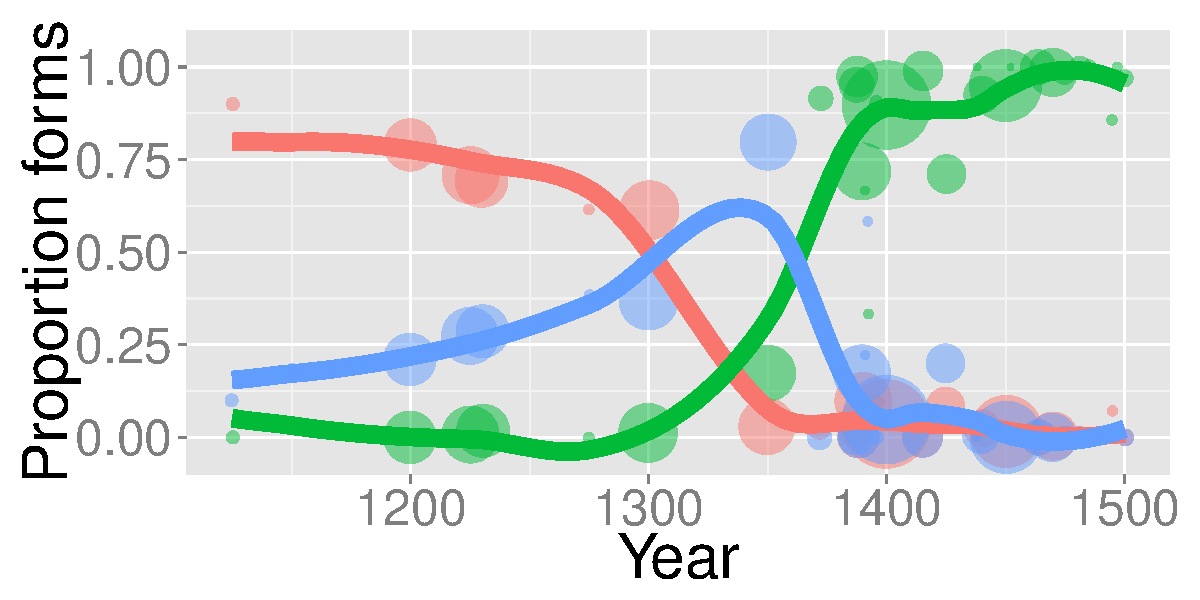
\includegraphics{neg-plot-auth}
\end{figure}

\section{}

\end{document}
